\documentclass[11pt,letterpaper]{article}
\usepackage[top=1in,bottom=1in,left=1in,right=1in]{geometry}
\usepackage[numbers]{natbib}      % http://merkel.zoneo.net/Latex/natbib.php
\usepackage{lmodern}
\renewcommand\familydefault{\sfdefault} 
\usepackage[T1]{fontenc}

%\bibpunct{(}{)}{;}{a}{,}{,}
\usepackage{chngpage}
\usepackage{stmaryrd}
\usepackage{amssymb}
\usepackage{amsmath}
\usepackage{amsthm}
\usepackage{graphicx}
\usepackage{lscape}
\usepackage{subfigure}
\usepackage{parskip}
\usepackage{algpseudocode}
\usepackage{algorithm}
\usepackage[usenames,dvipsnames]{color}
\usepackage{indentfirst}
\definecolor{myblue}{rgb}{0,0.1,0.6}
\definecolor{mygreen}{rgb}{0,0.3,0.1}
\usepackage[colorlinks=true,linkcolor=black,citecolor=mygreen,urlcolor=myblue]{hyperref}
\newcommand{\bocomment}[1]{\textcolor{Bittersweet}{[#1 -BTO]}}
\newenvironment{itemizesquish}{\begin{list}{\labelitemi}{\setlength{\parskip}{0.6cm}\setlength{\itemsep}{0em}\setlength{\labelwidth}{2em}\setlength{\leftmargin}{\labelwidth}\addtolength{\leftmargin}{\labelsep}}}{\end{list}}
\newcommand{\norm}[1]{\left\lVert#1\right\rVert}
\newcommand{\ignore}[1]{}
\let\oldReturn\Return
\renewcommand{\Return}{\State\oldReturn}
\newcommand\kcomment[1]{\textcolor{blue}{#1 - Khanh}}


\theoremstyle{definition}
\newtheorem{question}{Question}[section]

\setlength{\parindent}{30pt}
\linespread{1}

\title{
Protein sequence classification using neighbor-joining\\
   CMSC 701 Final report
}

\author{
	Khanh Nguyen and Ugur Koc
}

\begin{document}
\maketitle

\section{Introduction}

Neighbor-joining algorithm \cite{saitou1987neighbor} is a widely used algorithm for reconstructing phylogenetic trees from evolutionary distance data. The method takes a greedy bottom-up approach, iteratively joining pairs of taxonomic units that minimizes pre-computed distances. In this work, we present our C++ implementation of the algorithm and compare its running time with that of the PHYLIP package \cite{felsenstein2005phylip}, a popular open-source toolkit for inferring phylogenies. Experiments on synthesized data show that our implementation produces exactly same phylogenetic trees but runs twice as fast as the PHYLIP's implementation.  In addition, we test our implementation on a real phylogenetic dataset and provide a detailed benchmark on the accuracy of neighbor-joining algorithm under different distance metrics. We find that the algorithm produces the best trees when using the probability matrix from blocks (PMB) evolution model.

Our implementation is available at \url{https://github.com/ugur-koc/Neigbor-Joining}.

\section{Background}

%\subsection{Hierarchical clustering}

\subsection{Phylogenetic trees}

\begin{figure}[t]
  \centering
  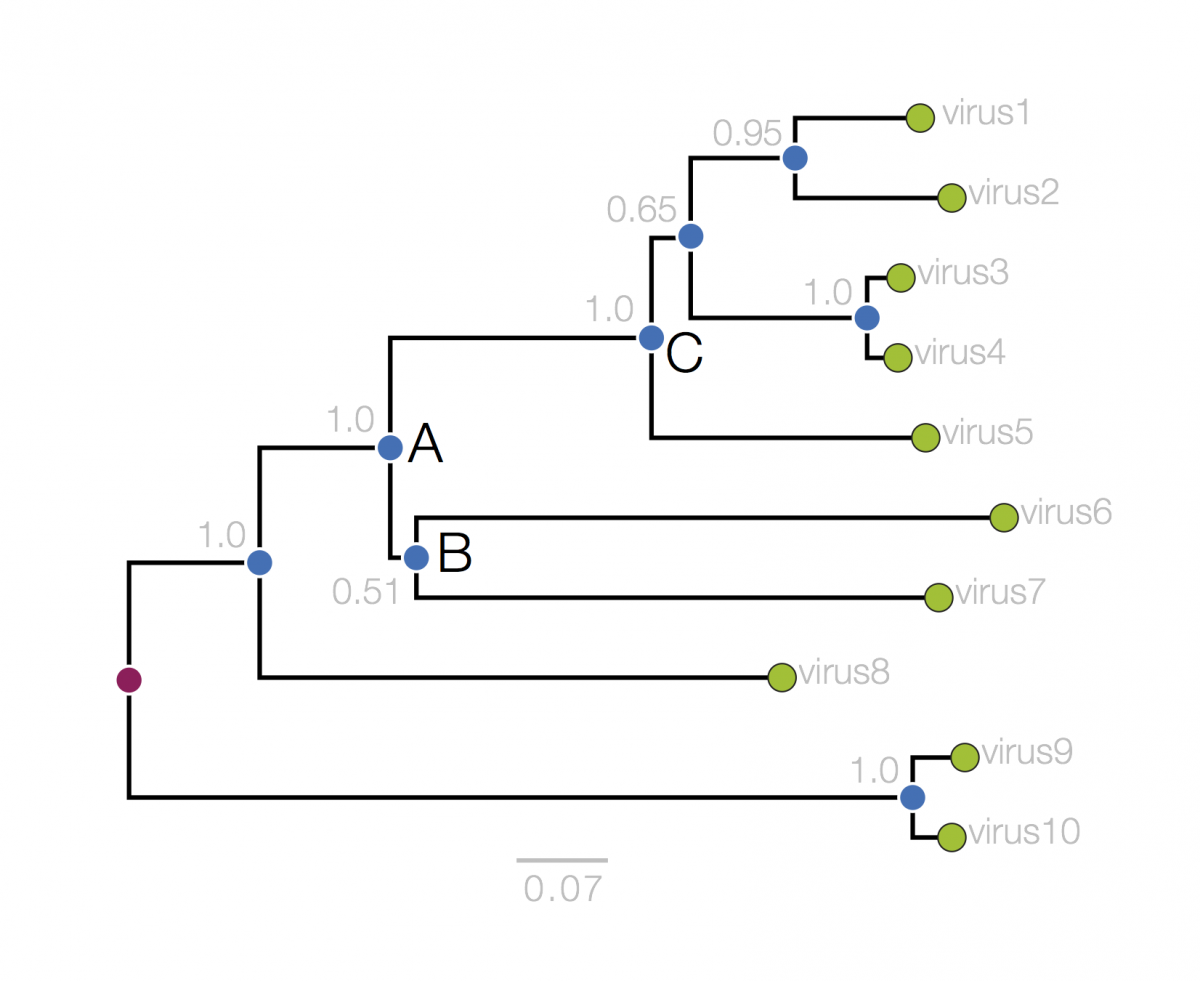
\includegraphics[width=0.5\textwidth]{phylogram_1a.png}
  \caption{An example of phylogenetic tree.}
  \label{fig:phytree}
\end{figure}

Phylogenetic trees are branching diagrams that show the evolutionary relationships between biological species. A weighted phylogenetic tree, with weights associated with its edges, captures the notion of genetic distances between species. By analyzing a weighted phylogenetic tree, we understand not only \textit{how} but also \textit{how much} species are related to or different from one another. Figure \ref{fig:phytree} \footnote{Image taken from \url{http://epidemic.bio.ed.ac.uk/how_to_read_a_phylogeny}} features an artificial phylogenetic tree of 10 viruses. Each virus is represented by a leave in the tree. Each internal node marks a milestone when a genetic divergence occurs. The lengths of the horizontal lines represent time periods. For instance, we can see that the divergence between virus 1 and virus 2 occurs before the divergence between virus 3 and virus 4. Phylogenetic trees can be constructed from various distance metrics. In this example, the metric assigned to the edges is the proportion of substitutions occurring on a sequence (the number of substitutions divided by the length of the sequence). 

\subsection{Neighbor-joining algorithm}

We consider the problem of constructing a phylogenetic tree from a set of protein sequences given their distance data. There are many approaches to tackle this problem. One approach frames the problem as a hierarchical clustering problem, which has been extensively studied in the fields of data mining or machine learning and has efficient solutions using statistical models. Although statistical approaches methods have been employed to build these complex evolution trees, classical approaches such as the NJ algorithm has the advantage of being easy to implement and scalable to large datasets. 

Figure \ref{alg:nj} summarizes the NJ algorithm. The input for the NJ algorithm are a set $P$ of sequences (usually DNA or protein sequences) and a distance matrix $D$ where each entry is the distance between a pair of sequences. The NJ algorithm constructs the phylogenetic tree from bottom up, going from leaves to root. It starts with a forest of $N$ single-node trees, each of which represents a sequence. In each later step, the algorithm selects two trees in the forest, joins them into a single tree by connecting their roots to a newly formed root. This process repeats until there is only tree left in the forest.

In an intermediate step, the algorithm decides which two trees to join by computing a \textit{branch length} matrix $L$ based on the distance matrix $D$. The branch length matrix contains $T \times T$ entries, where $T$ is the number of trees in the forest at the current step. Each entry of the matrix is computed as follows:  
\begin{equation}
  L_{i, j} = (T - 2) D_{i, j} - \sum_{k \in R}^n (D_{i, k} + D_{j, k})
  \label{eqn:branch}
\end{equation} where $R$ is the set of tree roots in the current forest.

Next, the algorithm selects the pair ($x$, $y$) with the highest branching length and connects each node to a new root, say $u$. The distances between u and x, y are:  
\begin{equation}
\begin{split}
  & D_{u, x}^{'} = \frac{1}{2} D_{x, y} + \frac{1}{2(T - 2)} \left[ \sum_{k \in R} (D_{x, k} - D_{y, k}) \right] 
\\  
& D_{u, y}^{'} = D_{x, y} - D_{u, x}^{'}
\end{split}
\label{eqn:distance_joined}
\end{equation}

We also update the distances between $u$ and other roots:
\begin{equation}
  D_{u, z}^{'} = \frac{1}{2} \left[ D_{x, z} + D_{y, z} - D_{x, y} \right], \ \ \ \text{for} \ z \neq x, y
\label{eqn:distance_nonjoined}
\end{equation}

\begin{figure}[t]
  \begin{algorithmic}[1]
    \Function{Neighor-joining}{$P$, $D$}
      \State $T \leftarrow \varnothing$ 
      \State $R \leftarrow P$
      \For {$t = 1 \dots |P| - 2$}
        \State $T \leftarrow |R|$
        \For {$(i, j) \in R \times R$}
          \State Compute $L_{i, j}$ using equation \ref{eqn:branch}. 
        \EndFor
        \State $(x, y) \leftarrow \arg \max L$
        \State Create new root $u$.
        \State Compute $D^{'}$ from $u$ to other nodes using equations \ref{eqn:distance_joined} and \ref{eqn:distance_nonjoined}.
        \State $D \leftarrow D^{'}$
        \State $T \leftarrow T \cup \{(u, x, D_{u, x}), (u, y, D_{u, y})\}$
        \State $R \leftarrow R \cup \{u\} \setminus \{x, y\}$
      \EndFor
    \State Let $u, v$ be the only two elements left in $R$.
    \State $T \leftarrow T \cup \{(u, v, D_{u, v})\}$
    \Return $T$
   \EndFunction
  \end{algorithmic}
  \caption{\label{alg:nj}The neighbor-joining algorithm.}
\end{figure}

The accuracy of the NJ algorithm largely depends on the accuracy of the distance metric used. Given an additive distance matrix, the NJ algorithm is guaranteed to construct a tree whose distances between species agree with it. 

\subsection{Computing distance matrix}\label{distance}

%Neighbor-joining algorithm is deterministic, i.e. given a distance matrix it will always produce the same phylogenetic tree. Therefore, computing accurate phylogenetic trees highly depends on the model of evaluation, i,e, distance matrix.

We experiment with two programs to generate the distance matrix:
\begin{enumerate}
	\item \textit{distmat} from the EMBOSS package \cite{rice2000emboss}  \footnote{\url{http://emboss.sourceforge.net/apps/release/6.6/emboss/apps/distmat.html}}: computes distance matrix for already aligned sequences based on various models (Junkes-Cantor, Tajima-Nei, etc.). We implement a wrapper script in Perl and then post-process the output distance matrix in order to feed it to our NJ implementation (see \textit{aligntodist.pl} in the code repository).
        \item \textit{protdist} from the PHYLIP package \footnote{\url{http://evolution.genetics.washington.edu/phylip.html}}: also computes distance matrix for aligned sequences We modify the tool's output format and remove unnecessary functionalities (see \textit{protdist.c} in the code repository).
\end{enumerate}

In addition to these programs, also computed distance matrix using global alignment scores for each pair of sequences. We write two scripts \textit{pairwisealignment.sh} and \textit{aligntodist\_pw.pl}. The former computes global alignment scores; the latter computes the distance matrix from those scores.

\section{Experiments}

We conduct two sets of experiments. For the first set, we compare our NJ implementation with that of another open-source NJ package in terms of both accuracy and running time. For the second set, we use various approaches for generating a distance matrix and compute phylogenetic trees from the matrices obtained. We then summarize and compare the running time and accuracy of each approach. 

%To evaluate the effectiveness and the efficiency of our implementations, we conducted a set of experiments. 

%We first aimed at generating accurate phylogenetic tree trying out different approaches (evaluation models) when generating the distance matrix. We then compared our results with some other popular implementations of neighbor-joining algorithm. 

%In these experiments, effectiveness refers to the accuracy of the phylogenetic tree produced at the end, i.e. how close/similar the tree to the ground truth by comparing them using robinson foulds symmetric difference \cite{robinson1981comparison}, and the efficiency refers to 1) the computation time of distance matrix and 2) computation of phylogenetic tree.

The distance matrices and phylogenetic trees computed from these experiments are available under the \textit{data} directory of our repository. 

\subsection{Data}

We use the \textit{85VASTdomains} dataset, which consists of 85 protein sequences of fully sequenced species representing all major Eukaryotic lineages \cite{khafif2014identification}. The longest sequence in this set consists of 125 amino acids. The ground-truth phylogenetic tree of these sequences has 9 major family branches. The sequences in this data have been aligned using multiple alignment techniques. In addition to this dataset, we also create a synthesized dataset consisting of 10 randomized distance matrices whose sizes vary from 100 to 1000. Each entry of each matrix is drawn from a uniform distribution over $[0, 1)$. The diagonals of the matrices are all zeros.   

\subsection{Results}

\subsubsection{Comparing with other neighbor-joining implementations}

\begin{figure}[t]
  \centering
  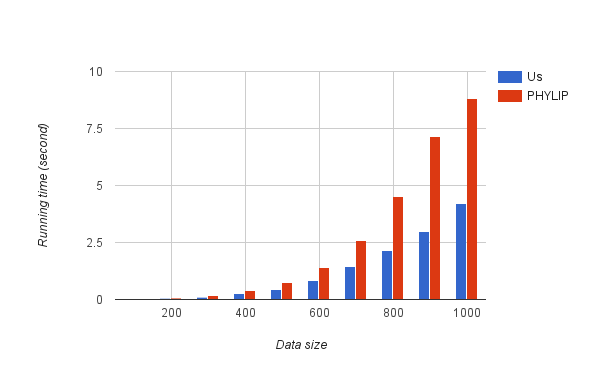
\includegraphics[width=0.8\textwidth]{runningtime.png}
  \caption{Comparison on the running times of our NJ implementation and PHYLIP's.}
  \label{fig:runningtime}
\end{figure}


We present comparisons between our NJ implementation and that of the PHYLIP package v3.6 \cite{felsenstein2005phylip}. PHYLIP provides a comprehensive set of implementations of various methods for inferring phylogenetic trees, including neighbor-joining and likelihood methods. We first run both NJ implementations on the \textit{85VASTdomains} dataset. We observe that they produces identical phylogenetic trees on this dataset. Next, we measure running times of the two implementations on the 10 synthesized datasets. As seen from Figure \ref{fig:runningtime}, our implementation outperforms the PHYLIP's implementation by a factor of approximately 2. This is a surprising result since we do not employ any advanced optimizing techniques in our implementation. We suspect the performance gain stems from optimizing features of the new C++11 compiler (we use g++ 4.9.2 with O2 optimizer whereas the PHYLIP package uses gcc 4.9.2 with no optimizing option).  

%TODO: What do you mean with "Our implementation produces the same phylogenetic tree on the dataset." it not clear!

\subsubsection{Compare approaches for generating distance matrices}

Here, we compare efficiency and accuracy of three different approaches mentioned in Section~\ref{distance} on the \textit{85VASTdomains} dataset. We do not compare sequence-aligning times in these experiments since we do not know how the dataset is aligned.
We use the norm of Robinson-Foulds symmetric difference (norm-rf) as the accuracy metric. This metric has been shown to be useful for comparing two phylogenetic trees \cite{robinson1981comparison}. It takes into account partitions that appear in only one of the trees. Therefore, the smaller the Robinson-Foulds symmetric difference metric, the similar trees are.

\begin{table}[h]
\centering
	\begin{tabular}{l|lll|lll|lll}
Gap Score	& \multicolumn{3}{c}{0} & \multicolumn{3}{c}{0.1} &  \multicolumn{3}{c}{1} \\
\hline
&	$T_d$	& $T_{NJ}$	& norm-rf &	$T_d$	& $T_{NJ}$	& norm-rf &	$T_d$	& $T_{NJ}$	& norm-rf \\
\hline
uncorrected		&	0.085	&	0.008	&	0.378	&	0.090	&	0.009	&	0.390	&	0.090	&	0.008	&	0.390	\\
Jukes-Cantor	&	0.091	&	0.008	&	0.366	&	0.090	&	0.010	&	0.354	&	0.096	&	0.009	&	0.463	\\
Kimura 	&	-	&	-	&	-	&	-	&	-	&	-	&	0.115	&	0.009	&	0.915	\\
\hline
\end{tabular}
\caption{Performance of evolution models implemented in \textit{distmat}. $T_d$: computation time of distance matrix (seconds); $T_{NJ}$: computation time of phylogenetic tree (seconds); norm-rf: Robinson-Foulds symmetric difference metric (smaller score is better).
}\label{tab:dist1}
\end{table}

\textbf{Performances of \textit{distmat} methods}. \textit{distmat} offers 3 different multiple substitution correction methods for aligned proteins sequences. They are \textit{uncorrected}, \text{Jukes-Cantor} \cite{jukes1969evolution}, and \textit{Kimura Protein} \cite{kimura1980simple}. We experiment with 3 gap score values (0, 0.1 and 1). Table~\ref{tab:dist1} presents computation times and norm-rf scores for these methods (Kimura protein evolution model does not make use of a gap score, thus we only give results in the last column).

\begin{table}[h]
\centering
	\begin{tabular}{l|lll}
	\hline
	&	$T_d$	& $T_{NJ}$	& norm-rf  \\
	\hline
	Dayhoff PAM	&	3.867	&	0.010	&	0.390	\\
	JTT			&	3.809	&	0.009	&	0.378	\\
	PMB			&	3.934	&	0.012	&	0.341	\\
	Kimura		&	0.013	&	0.012	&	0.963	\\
	\hline
	\end{tabular}
\caption{Performances of evolution models implemented in \textit{protdist}.}\label{tab:dist2}
\end{table}

\textbf{Performances of \textit{protdist} methods}. \textit{protdist} provides 5 methods for computing a distance matrix, but we only experiment with 4 of them \kcomment{Is there any reason for not experimenting with all 5?}. They are namely, \textit{Dayhoff PAM} \cite{kosiol2005different}, \textit{Jones-Taylor-Thornton} (JTT) \cite{jones1992rapid}, \textit{probability matrix from blocks} (PMB) \cite{veerassamy2003transition}, and \textit{Kimura's distance} \cite{kimura1983rare}. Table~\ref{tab:dist2} presents computation times and norm-rf scores for these methods.

\begin{figure}[t]
  s\centering
  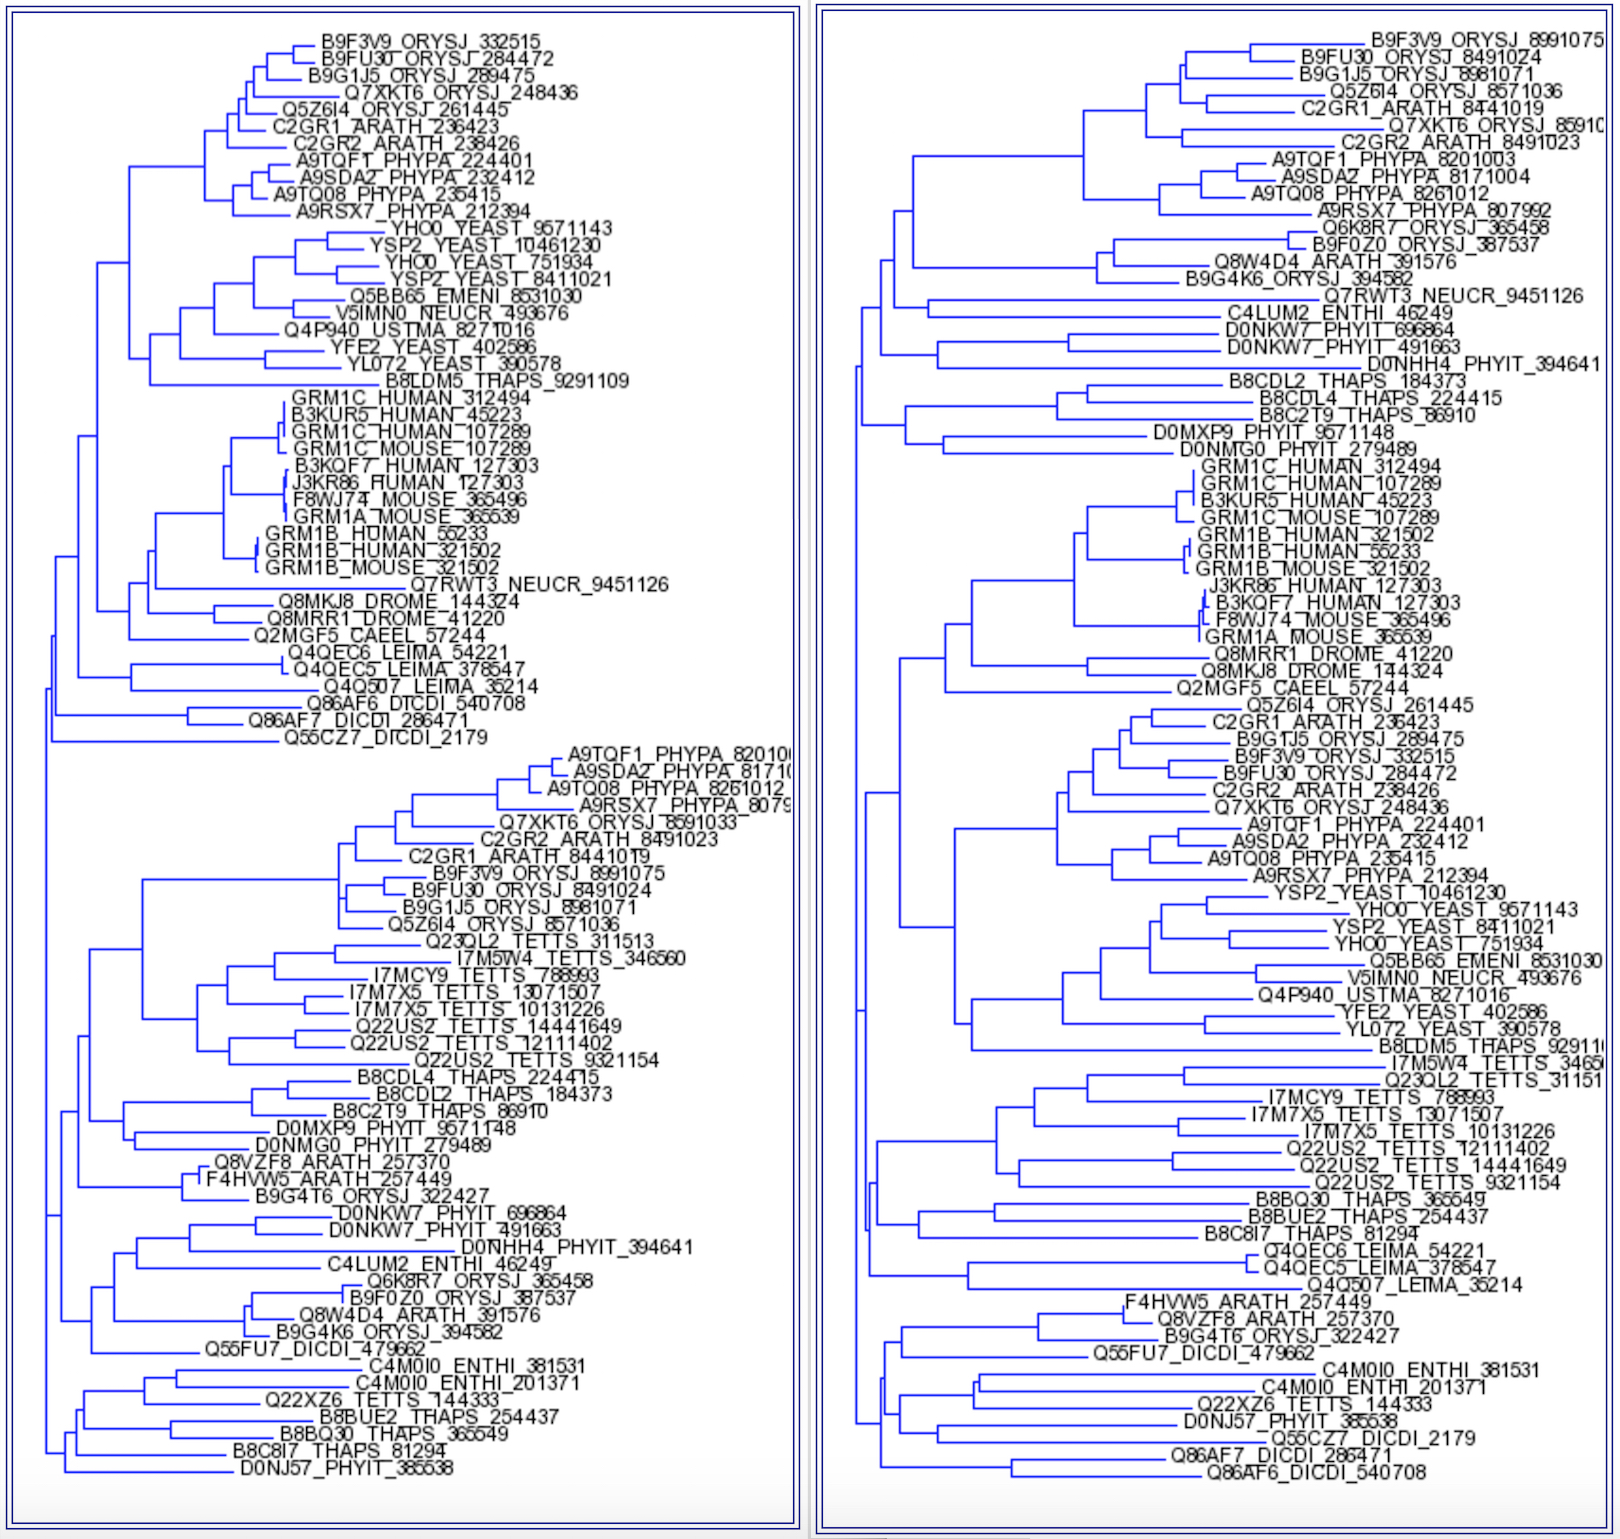
\includegraphics[width=0.9\textwidth]{gt-PMB.jpg}
  \caption{Ground truth phylogenetic tree (left) and phylogenetic tree generated from our implementation using PMB model (right).}
  \label{fig:gt-PMB}
\end{figure}

% I move this sentence to the DATA section
%For the tables above, the dataset we use was already aligned, i.e. multiple sequence alignment. 

\kcomment{Is the BLOSUM62 or EBLOSUM62?}
For the last part of this study we compute a global alignment score between each pair of sequences in this set. We use the EBLOSUM62 substitution matrix with gap penalty and gap extend penality set to 10.0 and 0.5, respectively. Since we want to assign higher scores to better alignments, we take the geometric inverse of the global alignment scores and then multiply them by 1000 to obtain the final distance scores.


Given the global alignment scores, computing the distance matrix takes 0.221 seconds ($T_d$), generating the phylogenetic tree takes using our NJ implementation takes 0.011 seconds ($T_{NJ}$). The norm-rf score of this tree is 0.634. 

Our results indicate that our NJ implementation is consistently efficient. Its performance does not depend on distance matrix generation approach. Accuracy however vary depending on the approach and the gap score. We obtain the best phylogenetic tree with PMB model (norm-rf=0.341). Figure \ref{fig:gt-PMB} shows the ground truth and our best tree side by side. 

\section{Concluding Remarks}

In this work, we provide a C++ implementation of the neighbor-joining algorithm. We compare our implementation with another well-known implementation on both real and synthesize data to demonstrate the correctness and efficiency of our implementation. Furthermore, we also evaluate the effectiveness of various distance metrics. Our results suggest that, for the dataset we work on, our implementation generates a highly accurate phylogenetic tree when it is combined with the PMB evolution model.
%and conducted experiments on a dataset of 85 protein sequences. We evaluated the effectiveness of our implementation by comparing our phylogenetic trees with the one report by Khafif et. al.~\cite{khafif2014identification}. We then evaluated the efficiency of our implementation by comparing the tree construction times with some other packages which are popular in the domain.


\bibliographystyle{plain}
\bibliography{report}

\end{document}
